
  \subsubsection{Front-end}
  \paragraph{Informazioni sul package}
    \begin{figure}[H] 
      \begin{center} 
        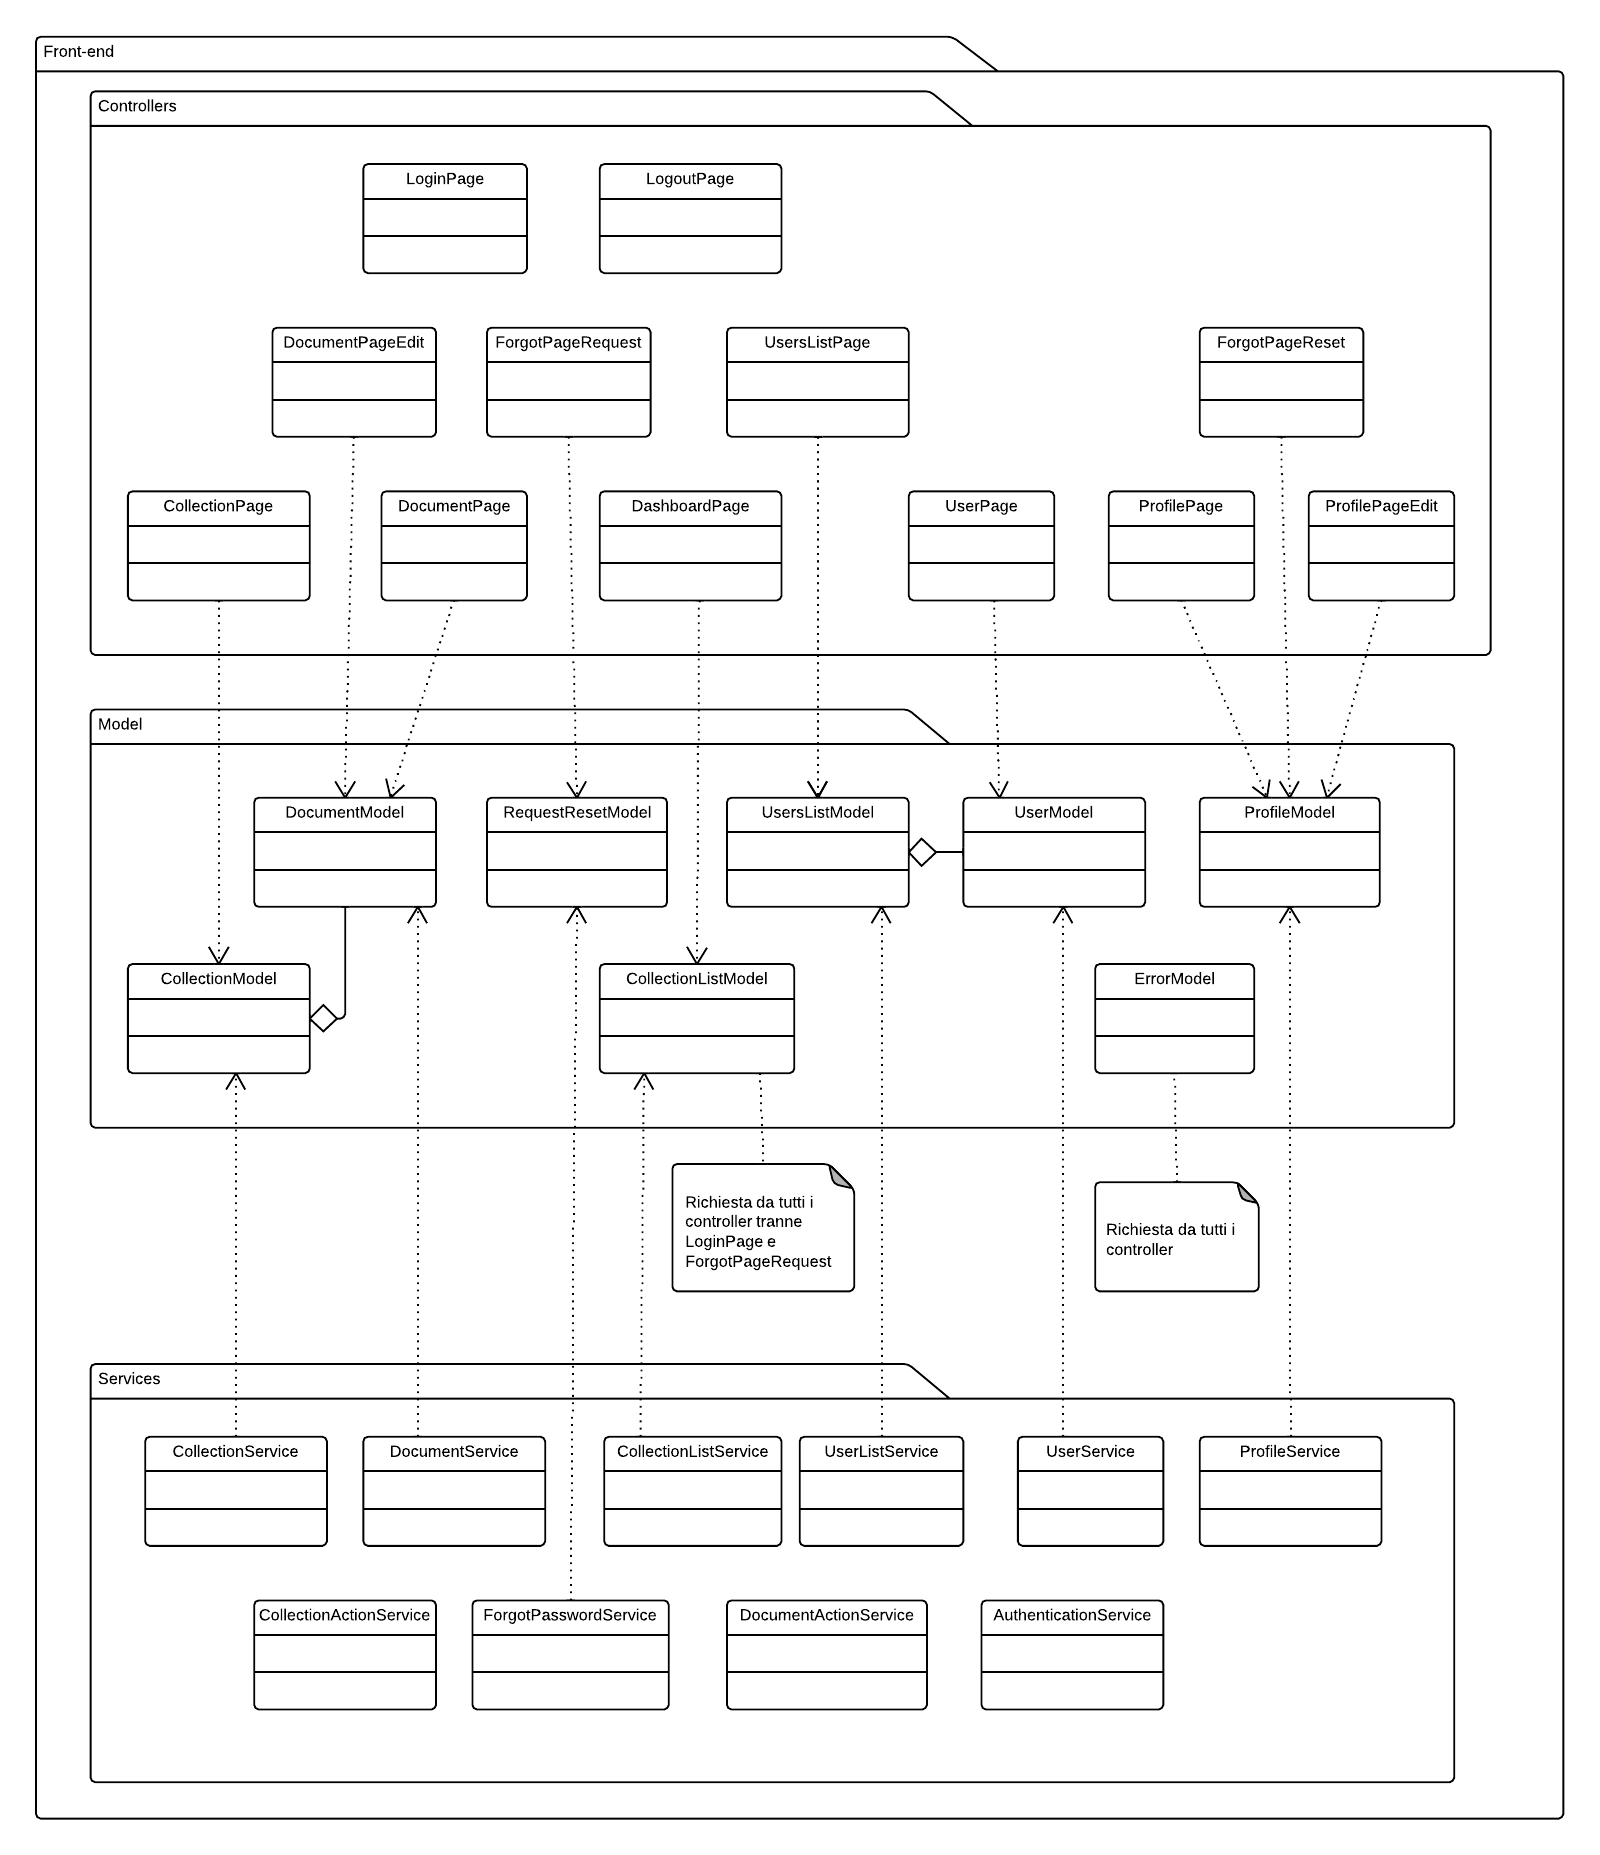
\includegraphics[width=\textwidth]{packages/Front-end.png}  
        \caption{Componente Front-end}
      \end{center}  
    \end{figure} 
  \subparagraph{Descrizione} 
    \begin{itemize}
    \item[] \glossario{Package} che racchiude tutta la componente di \glossario{Front-end}. Comprende il sottosistema che viene eseguito nei browser degli utenti e che fornisce l'interfaccia grafica all'utente non-tecnico che utilizzerà l'applicazione.
    \end{itemize} 
    \subparagraph{Package contenuti} 
    \begin{itemize}
        \item Front-end::Controllers
        \item Front-end::Services
        \item Front-end::Model
    \end{itemize}
  \subsubsection{Front-end::Controllers}
  \paragraph{Informazioni sul package}
    \begin{figure}[H] 
      \begin{center} 
        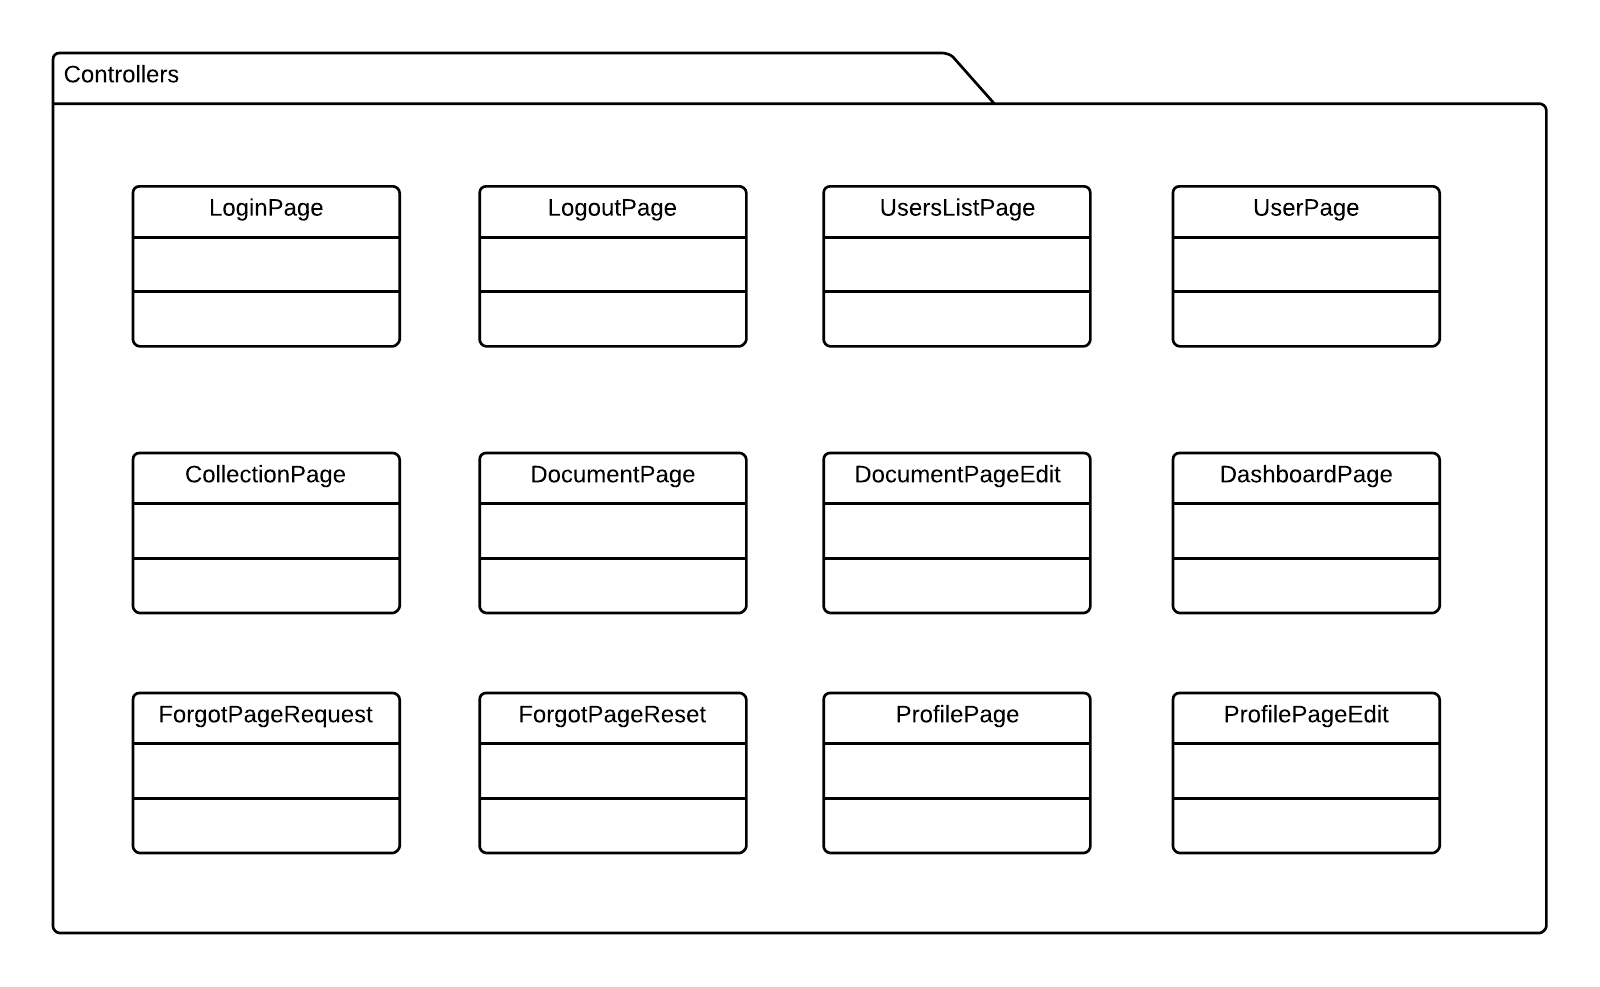
\includegraphics[width=\textwidth]{packages/Front-end::Controllers.png}  
        \caption{Componente Front-end::Controllers}
      \end{center}  
    \end{figure} 
  \subparagraph{Descrizione} 
    \begin{itemize}
    \item[] \glossario{Package} comprendente le classi che costituiscono i controller del componente \glossario{Front-end}. Ogni controller gestisce le operazioni e la logica applicativa riguardante una determinata pagina, e specifica quale view verrà utilizzata per la presentazione all'utente dei dati.
    \end{itemize} 
    \paragraph{Classi}
      \subparagraph{Front-end::Controllers::ForgotPageRequest}
        
        \textbf{\\ \\ Descrizione} 
          \begin{itemize}
            \item[] 
          \end{itemize}      
        \textbf{Utilizzo}  
          \begin{itemize}
            \item[] 
          \end{itemize}
      \subparagraph{Front-end::Controllers::ForgotPageReset}
        
        \textbf{\\ \\ Descrizione} 
          \begin{itemize}
            \item[] 
          \end{itemize}      
        \textbf{Utilizzo}  
          \begin{itemize}
            \item[] 
          \end{itemize}
      \subparagraph{Front-end::Controllers::LoginPage}
        
        \textbf{\\ \\ Descrizione} 
          \begin{itemize}
            \item[] Classe che gestisce le operazioni e la logica applicativa riguardante la pagina di Login.
          \end{itemize}      
        \textbf{Utilizzo}  
          \begin{itemize}
            \item[] Viene utilizzata per gestire il controllo sull'autenticazione di un utente.
          \end{itemize}
      \subparagraph{Front-end::Controllers::CollectionPage}
        
        \textbf{\\ \\ Descrizione} 
          \begin{itemize}
            \item[] Classe che gestisce le operazioni e la logica applicativa riguardante la pagina di gestione della Collection.
          \end{itemize}      
        \textbf{Utilizzo}  
          \begin{itemize}
            \item[] Utilizza la CollectionService per popolare correttamente lo scope con la lista di tutti i Document presenti nella Collection, e la CollectionActionService per gestire le azioni personalizzate sulla Collection.
          \end{itemize}
      \subparagraph{Front-end::Controllers::UsersListPage}
        
        \textbf{\\ \\ Descrizione} 
          \begin{itemize}
            \item[] Classe che gestisce le operazioni e la logica applicativa riguardante la pagina di gestione degli utenti.
          \end{itemize}      
        \textbf{Utilizzo}  
          \begin{itemize}
            \item[] Utilizza la UserListService per popolare correttamente lo scope fornendo quindi alla view la lista degli utenti.
          \end{itemize}
      \subparagraph{Front-end::Controllers::DashboardPage}
        
        \textbf{\\ \\ Descrizione} 
          \begin{itemize}
            \item[] Classe che gestisce le operazioni e la logica applicativa riguardante la pagina di gestione delle Collections.
          \end{itemize}      
        \textbf{Utilizzo}  
          \begin{itemize}
            \item[] Utilizza la CollectionListService per popolare correttamente lo scope fornendo quindi alla view la lista di tutte le Collections registrate.
          \end{itemize}
      \subparagraph{Front-end::Controllers::LogoutPage}
        
        \textbf{\\ \\ Descrizione} 
          \begin{itemize}
            \item[] Classe che gestisce l'operazione di logout di un utente.
          \end{itemize}      
        \textbf{Utilizzo}  
          \begin{itemize}
            \item[] 
          \end{itemize}
      \subparagraph{Front-end::Controllers::ProfilePageEdit}
        
        \textbf{\\ \\ Descrizione} 
          \begin{itemize}
            \item[] 
          \end{itemize}      
        \textbf{Utilizzo}  
          \begin{itemize}
            \item[] 
          \end{itemize}
      \subparagraph{Front-end::Controllers::UserPage}
        
        \textbf{\\ \\ Descrizione} 
          \begin{itemize}
            \item[] Classe che gestisce le operazioni e la logica applicativa riguardante la pagina profilo di un utente visualizzabile dall'admin.
          \end{itemize}      
        \textbf{Utilizzo}  
          \begin{itemize}
            \item[] Utilizza lo UserService per popolare correttamente lo scope fornendo quindi alla view i dati dell'utente.
          \end{itemize}
      \subparagraph{Front-end::Controllers::DocumentPageEdit}
        
        \textbf{\\ \\ Descrizione} 
          \begin{itemize}
            \item[] Classe che gestisce le operazioni di modifica di un Document.
          \end{itemize}      
        \textbf{Utilizzo}  
          \begin{itemize}
            \item[] Si occupa di prelevare i dati inseriti dall'admin nella view e utilizzando il DocumentService provvede a gestire la modifica delle informazioni riguardanti il Document.
          \end{itemize}
      \subparagraph{Front-end::Controllers::DocumentPage}
        
        \textbf{\\ \\ Descrizione} 
          \begin{itemize}
            \item[] Classe che gestisce le operazioni e la logica applicativa riguardante la pagina di gestione di un Document.
          \end{itemize}      
        \textbf{Utilizzo}  
          \begin{itemize}
            \item[] Utilizza il DocumentService per popolare correttamente lo scope fornendo quindi alla view la lista degli attributi del Document. \newline
Utilizza il DocumentActionService per gestire le azioni personalizzate sul Document.
          \end{itemize}
      \subparagraph{Front-end::Controllers::ProfilePage}
        
        \textbf{\\ \\ Descrizione} 
          \begin{itemize}
            \item[] Classe che gestisce le operazioni e la logica applicativa riguardante la pagina profilo di un utente.
          \end{itemize}      
        \textbf{Utilizzo}  
          \begin{itemize}
            \item[] Utilizza il ProfileService per popolare correttamente lo scope fornendo quindi alla view i dati dell'utente.
          \end{itemize}
  \subsubsection{Front-end::Services}
  \paragraph{Informazioni sul package}
    \begin{figure}[H] 
      \begin{center} 
        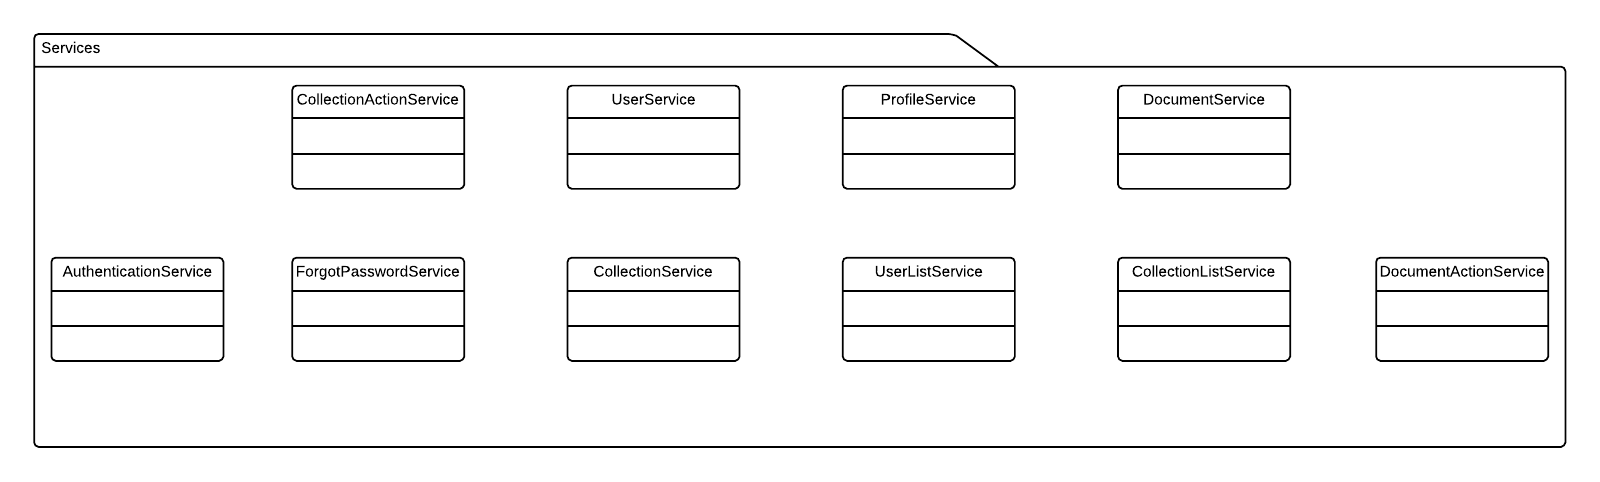
\includegraphics[width=\textwidth]{packages/Front-end::Services.png}  
        \caption{Componente Front-end::Services}
      \end{center}  
    \end{figure} 
  \subparagraph{Descrizione} 
    \begin{itemize}
    \item[] \glossario{Package} comprendente le classi che descrivono i meccanismi con cui il \glossario{Front-end} può interfacciarsi con le \glossario{API} del \glossario{Back-end}. Permette di recuperare i dati da inserire nel model e permette di azionare determinate procedure sul \glossario{Back-end} (per esempio la richiesta di recupero password o le ``action'' definite nel DSL).
    \end{itemize} 
    \paragraph{Classi}
      \subparagraph{Front-end::Services::AuthenticationService}
        
        \textbf{\\ \\ Descrizione} 
          \begin{itemize}
            \item[] Questa classe permette la creazione e l'eliminazione della sessione utente attraverso le corrispettive chiamate /login e /logout
          \end{itemize}      
        \textbf{Utilizzo}  
          \begin{itemize}
            \item[] La funzionalità offerta dalla classe è quella di poter fornire al Controller lo stato della sessione utente.
          \end{itemize}
      \subparagraph{Front-end::Services::UserService}
        
        \textbf{\\ \\ Descrizione} 
          \begin{itemize}
            \item[] Questa classe permette il recupero della risorsa REST rappresentante l'utente tramite la chiamata /users/$\{$user$\_$id$\}$
          \end{itemize}      
        \textbf{Utilizzo}  
          \begin{itemize}
            \item[] Le funzionalità offerte dalla classe sono: 
\begin{itemize} 
\item elenco dei dati relativi all'utente. 
\item modifica della password relativa al utente.
\item elevare o declassare un utente ad admin 
\item rimozione dell'utente. 
Tali funzionalità richiedono che l'utente sia un admin.
          \end{itemize}
          \textbf{Relazioni con altre classi}
          \begin{itemize}
              \item{Front-end::Model::UserModel}
          \end{itemize}
      \subparagraph{Front-end::Services::ProfileService}
        
        \textbf{\\ \\ Descrizione} 
          \begin{itemize}
            \item[] Questa classe permette il recupero delle risorsa REST rappresentante il profilo utente tramite la chiamata /profile
          \end{itemize}      
        \textbf{Utilizzo}  
          \begin{itemize}
            \item[] Le funzionalità offerte dalla classe sono:
\begin{itemize}
\item elenco dei dati relativi all'utente
\item modifica dei dati utente
\end{itemize}

Tali funzionalità richiedono che l'utente sia autenticato al sistema.
          \end{itemize}
          \textbf{Relazioni con altre classi}
          \begin{itemize}
              \item{Front-end::Model::ProfileModel}
          \end{itemize}
      \subparagraph{Front-end::Services::CollectionListService}
        
        \textbf{\\ \\ Descrizione} 
          \begin{itemize}
            \item[] Questa classe permette il recupero delle risorse REST rappresentanti le Collections tramite la chiamata /collections
          \end{itemize}      
        \textbf{Utilizzo}  
          \begin{itemize}
            \item[] La funzionalità offerta dalla classe è quella di poter fornire al Controller la lista delle Collections registrate dallo sviluppatore e presenti nel database delle collections.
Tale funzionalità richiede che l'utente sia registrato.
          \end{itemize}
          \textbf{Relazioni con altre classi}
          \begin{itemize}
              \item{Front-end::Model::CollectionListModel}
          \end{itemize}
      \subparagraph{Front-end::Services::DocumentActionService}
        
        \textbf{\\ \\ Descrizione} 
          \begin{itemize}
            \item[] Questa classe permette l'esecuzione (nel backend) delle azioni personalizzate di un Document tramite la chiamata /action/$\{$action name$\}$/$\{$collection name$\}$/$\{$document id$\}$
          \end{itemize}      
        \textbf{Utilizzo}  
          \begin{itemize}
            \item[] La funzionalità offerta dalla classe è quella di poter fornire al Controller il risultato dell'azione personalizzata definita dallo sviluppatore su un Document.
          \end{itemize}
      \subparagraph{Front-end::Services::CollectionActionService}
        
        \textbf{\\ \\ Descrizione} 
          \begin{itemize}
            \item[] Questa classe permette l'esecuzione (nel backend) delle azioni personalizzate di una Collection tramite la chiamata /action/$\{$action name$\}$/$\{$collection name$\}$
          \end{itemize}      
        \textbf{Utilizzo}  
          \begin{itemize}
            \item[] La funzionalità offerta dalla classe è quella di poter fornire al Controller il risultato dell'azione personalizzata definita dallo sviluppatore su una Collection.
          \end{itemize}
      \subparagraph{Front-end::Services::CollectionService}
        
        \textbf{\\ \\ Descrizione} 
          \begin{itemize}
            \item[] Questa classe permette il recupero della risorsa REST rappresentante la Collection tramite la chiamata  /collection/$\{$collection$\_$name$\}$
          \end{itemize}      
        \textbf{Utilizzo}  
          \begin{itemize}
            \item[] La  funzionalità offerta dalla classe è quella di poter fornire al Controller la lista di Document presenti nella Collection.
          \end{itemize}
          \textbf{Relazioni con altre classi}
          \begin{itemize}
              \item{Front-end::Model::CollectionModel}
          \end{itemize}
      \subparagraph{Front-end::Services::UserListService}
        
        \textbf{\\ \\ Descrizione} 
          \begin{itemize}
            \item[] Questa classe permette il recupero delle risorse REST rappresentanti gli utenti registrati all'applicazione tramite la chiamata /users
          \end{itemize}      
        \textbf{Utilizzo}  
          \begin{itemize}
            \item[] La funzionalità offerta dalla classe è quella di poter fornire al Controller la lista degli utenti presenti nel database delle credenziali.
Tale funzionalità richiede che l'utente sia un admin.
          \end{itemize}
          \textbf{Relazioni con altre classi}
          \begin{itemize}
              \item{Front-end::Model::UsersListModel}
          \end{itemize}
      \subparagraph{Front-end::Services::DocumentService}
        
        \textbf{\\ \\ Descrizione} 
          \begin{itemize}
            \item[] Questa classe permette il recupero delle risorse REST rappresentanti i Document di una Collection tramite la chiamata /collections/$\{$collection$\_$name$\}$/$\{$document id$\}$
          \end{itemize}      
        \textbf{Utilizzo}  
          \begin{itemize}
            \item[] Le funzionalità offerte dalla classe sono: 
\begin{itemize} 
\item elenco dei dati relativi al Document 
\item modifica dei dati relativi al Document
\item rimozione del Document 
\end{itemize} 
Tali funzionalità richiedono che l'utente sia autenticato al sistema.
          \end{itemize}
          \textbf{Relazioni con altre classi}
          \begin{itemize}
              \item{Front-end::Model::DocumentModel}
          \end{itemize}
      \subparagraph{Front-end::Services::ForgotPasswordService}
        
        \textbf{\\ \\ Descrizione} 
          \begin{itemize}
            \item[] Questa classe si occupa di inviare al server una richiesta di recupero password tramite la chiamata /password/lost e la conseguente modifica attraverso la chiamata /password/reset.
          \end{itemize}      
        \textbf{Utilizzo}  
          \begin{itemize}
            \item[] La  funzionalità offerta dalla classe è quella di interagire col server delegando quest'ultimo all'invio di una mail all'utente per il recupero della password e successivamente alla sua modifica.
          \end{itemize}
          \textbf{Relazioni con altre classi}
          \begin{itemize}
              \item{Front-end::Model::RequestResetModel}
          \end{itemize}
  \subsubsection{Front-end::Model}
  \paragraph{Informazioni sul package}
    \begin{figure}[H] 
      \begin{center} 
        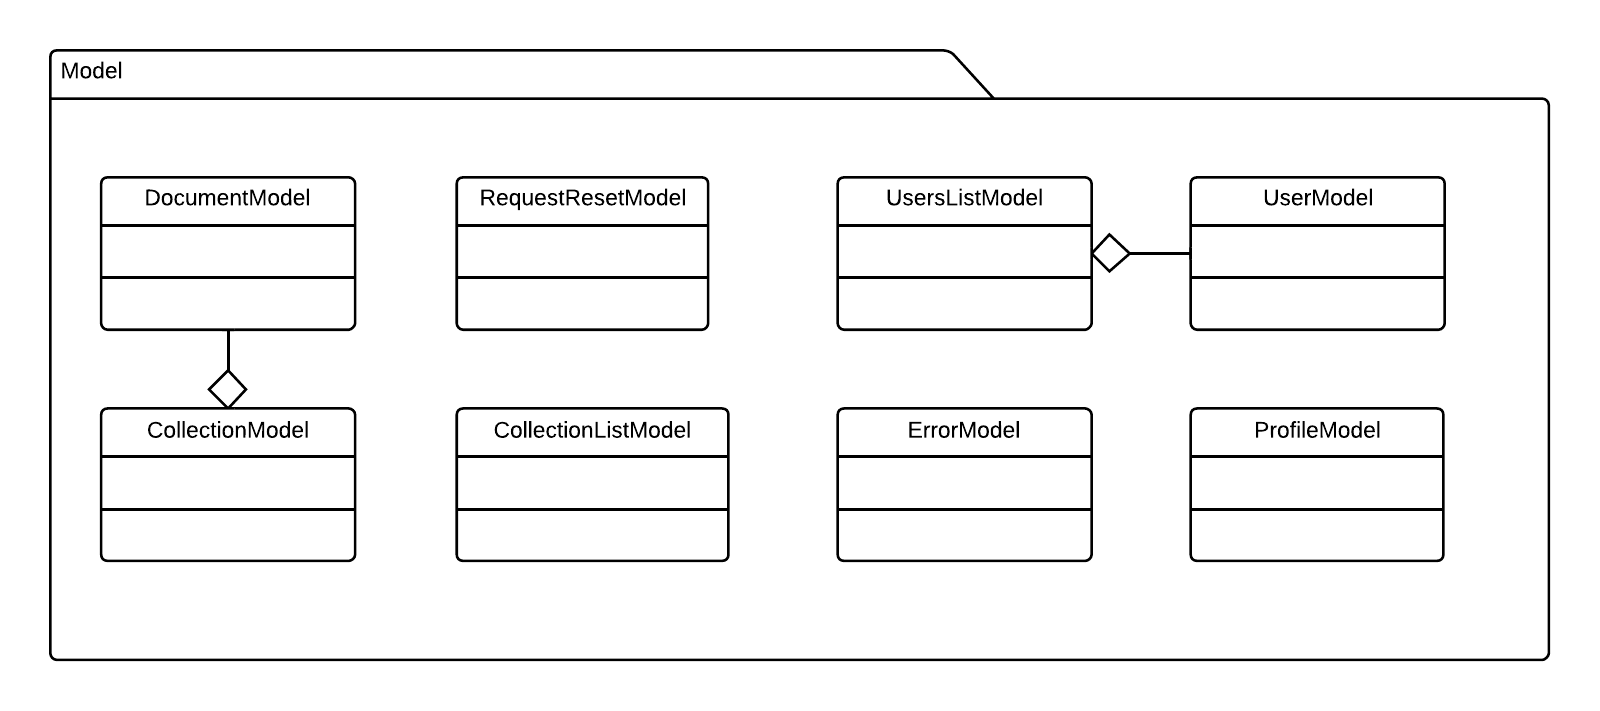
\includegraphics[width=\textwidth]{packages/Front-end::Model.png}  
        \caption{Componente Front-end::Model}
      \end{center}  
    \end{figure} 
  \subparagraph{Descrizione} 
    \begin{itemize}
    \item[] \glossario{Package} che comprende le classi dei modelli dei dati utilizzati dal \glossario{Front-end}. Servono a fornire ai controller e ai service le informazioni su quali campi potranno aspettarsi negli oggetti che arrivano tramite le \glossario{API} del \glossario{Back-end}.

Le classi di questo \glossario{package} sono state progettate, ma si prevede che non verranno codificate poiché verrà sfruttato lo stile di \glossario{duck-typing} della gestione dei tipi di \glossario{JavaScript}.
    \end{itemize} 
    \paragraph{Classi}
      \subparagraph{Front-end::Model::ErrorModel}
        
        \textbf{\\ \\ Descrizione} 
          \begin{itemize}
            \item[] E la classe che rappresenta il modello dati dell'errore.
          \end{itemize}      
        \textbf{Utilizzo}  
          \begin{itemize}
            \item[] Utilizzato da tutti i controller per poter accedere alle informazioni riguardanti l'errore.
          \end{itemize}
      \subparagraph{Front-end::Model::CollectionListModel}
        
        \textbf{\\ \\ Descrizione} 
          \begin{itemize}
            \item[] E la classe che rappresenta la struttura dati delle Collections.
          \end{itemize}      
        \textbf{Utilizzo}  
          \begin{itemize}
            \item[] Fornisce una rappresentazione sotto forma di oggetto delle informazioni scambiate con il back-end e permette alla CollectionListService e alla DashboardPage Controller di poter accedere alla lista delle Collections.
          \end{itemize}
      \subparagraph{Front-end::Model::RequestResetModel}
        
        \textbf{\\ \\ Descrizione} 
          \begin{itemize}
            \item[] E il modello che contiene i dati dell'utente che richiede un recupero della password.
          \end{itemize}      
        \textbf{Utilizzo}  
          \begin{itemize}
            \item[] Fornisce una rappresentazione sotto forma di oggetto delle informazioni scambiate con il back-end e permette al ForgotPasswordService e al ForgotPageRequest Controller di poter accedere ai dati dell'utente.
          \end{itemize}
      \subparagraph{Front-end::Model::UsersListModel}
        
        \textbf{\\ \\ Descrizione} 
          \begin{itemize}
            \item[] E la classe che rappresenta la struttura dati dell'utente.
          \end{itemize}      
        \textbf{Utilizzo}  
          \begin{itemize}
            \item[] Fornisce una rappresentazione sotto forma di oggetto delle informazioni scambiate con il back-end e permette allo UserListService e allo UserListPage Controller di poter accedere alla lista degli utenti.
          \end{itemize}
      \subparagraph{Front-end::Model::UserModel}
        
        \textbf{\\ \\ Descrizione} 
          \begin{itemize}
            \item[] E la classe che rappresenta la struttura dati dell'utente.
          \end{itemize}      
        \textbf{Utilizzo}  
          \begin{itemize}
            \item[] Fornisce una rappresentazione sotto forma di oggetto delle informazioni scambiate con il back-end e permette allo UserService e allo UserPage Controller di poter accedere agli attributi dell'utente.
          \end{itemize}
      \subparagraph{Front-end::Model::DocumentModel}
        
        \textbf{\\ \\ Descrizione} 
          \begin{itemize}
            \item[] E la classe che rappresenta la struttura dati dei Document relativi ad una Collection.
          \end{itemize}      
        \textbf{Utilizzo}  
          \begin{itemize}
            \item[] Fornisce una rappresentazione sotto forma di oggetto delle informazioni scambiate con il back-end e permette al DocumentService e al DocumentPage Controller di poter accedere agli attributi del Document.
          \end{itemize}
      \subparagraph{Front-end::Model::CollectionModel}
        
        \textbf{\\ \\ Descrizione} 
          \begin{itemize}
            \item[] E la classe che rappresenta il modello delle Collection.
          \end{itemize}      
        \textbf{Utilizzo}  
          \begin{itemize}
            \item[] Fornisce una rappresentazione sotto forma di oggetto delle informazioni scambiate con il back-end e permette alla CollectionService e alla CollectionPage Controller di poter accedere alla lista delle Collections.
          \end{itemize}
      \subparagraph{Front-end::Model::ProfileModel}
        
        \textbf{\\ \\ Descrizione} 
          \begin{itemize}
            \item[] E la classe che rappresenta la struttura dati dell'utente.
          \end{itemize}      
        \textbf{Utilizzo}  
          \begin{itemize}
            \item[] Permette al ProfileService di avere una rappresentazione delle informazioni dell'utente da scambiare con il back-end, al ProfilePage Controller e al ProfileEditController per ottenere il dati dell'utente da visualizzare nella view della pagina profilo e al ForgotPageReset Controller per la modifica della password.
          \end{itemize}